\documentclass[11pt,b5paper, titlepage]{report}
\usepackage{amssymb}
\usepackage{amsmath}
\usepackage{graphicx} %figures, \includegraphics[attr1=val1, attr2=val2, ..., attrn=valn]{imagename}
\usepackage{comment} %multi-line commenting, \begin{comment}, end{comment}
\usepackage{wrapfig} %to wrap text around figure  (in deformableModels)
\usepackage[lmargin=25mm,rmargin=25mm,tmargin=27mm,bmargin=30mm]{geometry}
\usepackage[hidelinks]{hyperref}
\usepackage{caption} %to be able to do linebreak inside captions, and more
\usepackage[bottom]{footmisc}

\newcommand{\indentitem}{\setlength\itemindent{25pt}} 
%instead of writing {\setlength\itemindent{25pt} to indent an item inside the itemize envirnment, {\indentitem} can now be used..see last section in the chapter about level set method

%modify date format (used in titlepage)
\usepackage{datetime}
\renewcommand{\dateseparator}{.}
\ddmmyyyydate
	
\begin{document}

%\input{forside}

% Set the page numbers to be roman, starting at page 1
\pagestyle{headings}
\setcounter{page}{1}
\pagenumbering{roman}

%\begin{abstract}
%TODO
%\end{abstract}

\tableofcontents
\listoffigures
%\listoftables ikke vits for bare en table
%\clearpage

% set the page numbers to be arabic, starting at page 1 %
\setcounter{page}{1}
\pagenumbering{arabic}

%input each chapter
\section{Segmentation}
Image segmentation is the process of dividing an image into meaningful non-overlapping regions or objects. The main goal is to divide an image into parts that have strong correalation with objects of the real world. Segmented regions are homogenous according to some property, such as pixel intensity or texture. Mathematically speaking, a complete segmentation of an image I is a finite set of regions \(I_1,...., I_S\) such that the condition (from \cite{drung00})
\begin{equation}
I = \bigcup_{i=1}^S I_{i} , \quad I_{i} \cap I_{j} = \emptyset , \quad i \neq j
\label{segCond}
\end{equation}
is satisfied. Image segmentation is one of the first steps leading to image analysis and interpretation. It is used in many different fields, such as machine vision, biometric measurements and medical imaging.

Automated image segmentation is a challenging problem for many different reasons. Noise, partial occluded regions, missing edges, lack of texture contrast between regions and background are some of the reasons. Noise is an artifact often found in images which makes the segmentation process harder. In the process of generating medical images noise is often introduced by the capturing devices. As a pre-processing step before segmentation the image can be smoothed to reduce noise. In the context of medical images segmentation usually means a delineation of anatomical structures. This is important for e.g. measurements of volume or shape. Low level segmentation methods are usually not good enough to segment medical images. Thus, higher level segmentation methods that are more complex and gives better results are used. The biggest difference between low-level segmentation methods and higher level segmentation methods is the use of apriori information. Low-level methods usually have no information about the image to be segmented, while high-level segmentation methods can incorporate different types and amount of apriori information.

Traditional low-level image segmentation methods can roughly be divided according to the type of technique used:
\begin{itemize}
  \item Global/Histogram based methods
  \item Region based methods
  \item Edge based methods
\end{itemize}

\subsection{Histogram-based segmentation methods}
Global knowledge about an image is usually represented by the histogram of the intensity values in the image. Histogram-based segmentation methods uses this information to segment simple images. These segmentation methods are usually much faster than other methods, but restricted to images with simple features. 

\subsubsection{Thresholding}
The simplest segmentation approache is called thresholding. Thresholding is used to seperate objects from the background using a threshold value \(T\). A threshold value splits the image in two groups, where all pixels with intensity value higher than \(T\) represents an object or the foreground, and the rest represents another object or the background. Choosing a good thresold value is important, as small changes in the value can significantly affects the resulting segmentation, which can be seen in figure \ref{thresholding}c and \ref{thresholding}d (described in more detail later). The threshold can be selected manually by either inspecting the image or the histogram of the image. But usually the threshold is selected automatically, and a variety of methods for automatically selecting \(T\) exists. When little noise is present, the mean or median intensity values can be selected as the threshold. The simplest method to select a threshold, apart from doing it manually, is iterative thresholding and is computed as follows:
\begin{enumerate}
\item Choose an initial threshold \(T_{0}\) and segment the image.
\item The segmented image will consist of two groups, \(C_{1}\) and \(C_{2}\). Set the new threshold value \(T_{i}\) to be the sum of the mean intensity values from \(C_{1}\) and \(C_{2}\), divided by 2.
\item Segment the image using \(T_{i}\).
\item Repeat steps 2 and 3 until \(|T_{i} - T_{i-1}|\) is less than a predefined value.
\end{enumerate}
 
By using multiple threshold values the image can be split up into several regions. Segmentation by thresholding is only suitable for very simple images, where the objects in the image does not overlap and their intensity values are clearly distinct from the background intensity values. If the threshold is poorly chosen, the resulting binary image would not be able to correctly distinguish the foreground from the background.  

\subsubsection{Otsu's thresholding method}
Otsu's thresholding method assumes that the image contains two regions with the values in each region creating a cluster. Otsu's method tries to make each cluster (or class) as tight as possible, thus minimizing their overlap. The goal then is to select the threshold that minimizes the combined spread. The threshold that maximizes the between-class variance \(\sigma_{b}^2(t) = \omega_{1}(t)\omega_{2}(t)\,[\mu_{1}(t)\mu_{2}(t)]^2\) is sought after. \(\omega_{1}(t)\) and \(\omega_{2}(t)\) are the weights (computed from the normalized histogram) of the two clusters, and \(\mu(t)\) is the mean intensity value of the clusters. Otsu's method starts by splitting the histogram into two clusters using an initial threshold. Then \(\sigma_{b}^2(t)\) is computed for that threshold value. The between-class variance \(\sigma_{b}^2(t)\) is then iteratively computed for every intensity value, and the threshold that maximizes the between-class variance \(\sigma_{b}^2(t)\) (or minimizes the within-class variance) is chosen as the final threshold value.

Figure \ref{thresholding} illustartes a gray-scale image and the segmentation results using both iterative global thresholding and Otsu's method. The threshold found using the iterative threshold method is 0.7332 where the range is from 0 (black) to 1 (white). The threshold found using Otsu's method is 0.7686. The image to be segmented is shown in figure \ref{thresholding}a, and its histogram in figure \ref{thresholding}b. As can be seen from the histogram, it is not possible to select a near perfect threshold by just looking at it. Figure \ref{thresholding}c illustrates the segmentation result from the iterative global thresholding method and figure \ref{thresholding}d is the segmentation result using Otsu's method. Even though the difference of the two threshold values is small, the segmentation results have a considerable difference, where Otsu's method gives a better result.

\begin{figure}[h!]
\centering
\begin{minipage}{.45\textwidth}
\begin{tabular}{c}
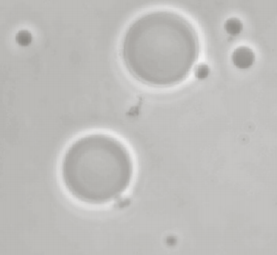
\includegraphics[width=.9\textwidth]{backgroundTheory/segmentation/NotSegmented} \\
(a)
\end{tabular}
\end{minipage}
\begin{minipage}{.45\textwidth}
\begin{tabular}{c}
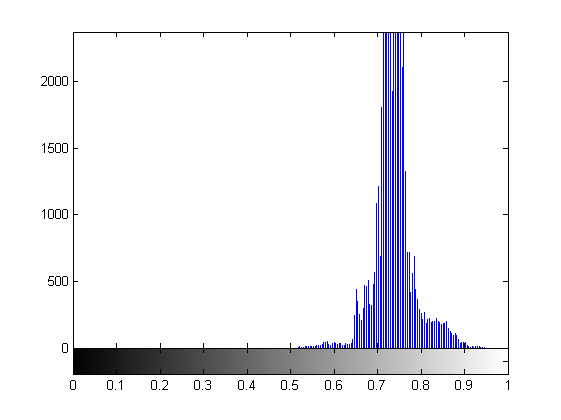
\includegraphics[width=.9\textwidth]{backgroundTheory/segmentation/NotSegmentedHist} \\
(b)
\end{tabular}
\end{minipage}
\\
\begin{minipage}{.45\textwidth}
\begin{tabular}{c}

\includegraphics[width=.9\textwidth]{backgroundTheory/segmentation/globalThresholded} \\
(c)
\end{tabular}
\end{minipage}
\begin{minipage}{.45\textwidth}
\begin{tabular}{c}

\includegraphics[width=.9\textwidth]{backgroundTheory/segmentation/otsuThresholded} \\
(d)
\end{tabular}
\end{minipage}
\caption{(a): Image to be segmented, (b): Histogram of image, (c): Segmented using iterative global thresholding, with $T = 0.7332$, (d): Segmented using Otus's method with $T = 0.7686$.}
\label{thresholding}
\end{figure}

\subsection{Region based segmentation}
Region based segmentation methods tries to find homogenous regions based on gray-scale, color, texture or any other pixel based measure in an image. Pixels with similar properties are grouped together in regions \(I_i\). The choice of homogenity criteria is an important factor that affects the end segmentation result. In addition to the condition in equation \ref{segCond}, images segmented by region based segmentation also satisfies the two following conditions:
\begin{itemize}
  \item All regions \(I_i\) should be homogenous according to some specified criteria: \(H(I_i) = true, \ i=1,2,...,S.\) \label{test}
  \item The region that results from merging two adjacent regions \(R_i\) and \(R_j\) is not homogenous: \(H(I_i \cup I_j) = false. \label{test2} \) 
\end{itemize}
An example of a homogenity criteria for a region could be all adjacent pixels with intensity value within a range \(\{x,y|x \pm y\}\). That is, if two adjacent pixels have intensity values in the range \(x \pm y\) they are in the same region. Region based segmentation methods are usually better than edge based segmentation methods in noisy images where the borders are difficult to detect. 

\subsubsection{Region growing}
An example where thresholding is insuficient is when parts of the foreground
have the same pixels values as part of the background. In this case, region
growing can be used. Region growing starts at a point (seed point) defined
to be inside the forground and grows to include neighbouring foreground
pixels. This seed point is manually set at the beginning and consiste of one
or more pixels. A small region of 4x4 or 8x8 can for example be chosen as a seed region. The regions described by the seed points grows by merging with their neighbouring points (or regions) if the homogenity criteria is met. This merging is continued until merging any more would violate the homogenity criteria. When a region cannot be merged with any of its neighbours it is marked as final, and when all regions are marked as final the segmentation is completed. The result of region growing can depend on the order in which the regions are merged. Thus, the segmentation result may differ if the segmentation begins, for example, in the top right corner or the lower left corner. This is because the order of the merging can cause two similar adjacent regions \(R_1\) and \(R_2\) not to be merged if an earlier merge of \(R_1\) and \(R_3\) changed the characteristics of \(R_1\) such that it no longer is similar (enough) to \(R_2\). 

\subsubsection{Region splitting}
Region splitting is the opposite of region growing, and starts with a single region covering the whole image. This region is iteratively split into smaller regions until all regions are homogenous according to a homogenity criteria. One disadvantage of both region growing and region splitting is that they are sensitive to noise, resulting in regions that should be merged remaining unmerged, or merging regions that should not be merged.

\subsection{Edge based segmentation}
Edge based segmentation methods are used to find edges in the image by detecting intensity changes. The edge magnitude at a certain point is the same as the gradient magnitude, and the edge direction is perpendicular to the gradient. Thus, change in intensity at a point can be detected by using first and second order derivatives. There are various edge detection operators, and they all approximate a scalar edge value for each pixel in an image based on a collection of weights applied to the pixel and its neighbours. These operators are usually represented as rectangular masks or filters consisting of a set of weight values. These masks are applied to the image to be segmented using discrete convolution. 

\subsubsection{First and second order operators}
A simple second order edge detection operator is the Laplacian operator, based on the Laplacian equation:
\begin{equation}
\nabla^2f(x,y) = \frac{\partial^2 f}{\partial x^2} + \frac{\partial^2 f}{\partial y^2}
\end{equation}
This equation measures edge magnitude in all directions and is invariant to rotation of the image. Second order derivatives are commonly discretized by approximating it as \(\frac{\partial^2 f}{\partial x^2} = f(x+1,y) + f(x-1,y) - 2f(x,y)\) which is also how the Laplacian is discretized: 
\begin{equation}
\nabla^2f(x,y) = f(x+1,y) + f(x-1,y) + f(x,y+1) + f(x,y-1) - 4f(x,y)
\end{equation}
This Laplacian equation is represented by the mask in equation \ref{laplacianMask1}, and a variant of the equation that also takes into account diagonal elements is shown in \ref{laplacianMask2}.
\newline
\newline 
\begin{minipage}{.45\textwidth}
\begin{equation}
\begin{pmatrix}
0 & 1 & 0 \\
1 & -4 & 1 \\
0 & 1 & 0
\end{pmatrix}
\label{laplacianMask1}
\end{equation}
\end{minipage}
\begin{minipage}{.45\textwidth}
\begin{equation}
\begin{pmatrix}
1 & 1 & 1 \\
1 & -8 & 1 \\
1 & 1 & 1
\end{pmatrix}
\label{laplacianMask2}
\end{equation}
\end{minipage}
\newline
\newline

Since the Laplacian mask is based on second order derivatives it is very sensitive to noise. Moreover, it produces double edges and is not able to detect the edge direction. The center of the actual edge can be found by finding the zero-crossing between the double edges. Hence, the Laplacian is usually better then first order derivatives to find the center-line in thick edges. To overcome the sensitivity to noise problem, the image can be smoothed beforehand. This is the idea behind the Laplacian of Gaussian (LoG) operator. The LoG mask is a combination of a Gaussian operator (which is a smoothing mask) and a Laplacian mask. By convolving an image with a LoG mask it is smoothed at the same time as edges are detected. The smoothness is determined by the standard deviation of the Gaussian, which also determines the size of the LoG mask.

There are various masks based on first order derivatives, and two of them are the Prewitt and Sobel masks, represented in equation \ref{prew} and \ref{sobel} respectively. These two are not rotation invariant, but the masks can be rotated to emphasize edges of different directions. The masks as they are represented in equation \ref{prew} and \ref{sobel} highlights horizontal edges.
\newline
\newline
\begin{minipage}{.45\textwidth}
\begin{equation}
\begin{pmatrix}
1 & 1 & 1 \\
0 & 0 & 0 \\
-1 & -1 & -1
\end{pmatrix}
\label{prew}
\end{equation}
\end{minipage}
\begin{minipage}{.45\textwidth}
\begin{equation}
\begin{pmatrix}
1 & 2 & 1 \\
0 & 0 & 0 \\
-1 & -2 & -1
\end{pmatrix}
\label{sobel}
\end{equation}
\end{minipage}
\newline
\newline
As can be seen from the above masks, the only difference between the Sobel and Prewitt is that the middle column (or row in a rotated version) in the Sobel mask is weighted by 2 and -2. This results in smoothing since the middle pixel is given more importance, hence, the Sobel is less sensitive to noise than Prewitt. 

Figure \ref{edgeSeg}a illustrates a gray-scale image and \ref{edgeSeg}b is the edge segmented image based on LoG. \ref{edgeSeg}c is the edge image resulted from the Sobel mask in equation \ref{sobel}b and \ref{edgeSeg}d is the result from segmentation after rotating the mask \(90^\circ\). The segmentations resulted by using the Prewitt operator to segment the image in figure \ref{edgeSeg}a had no significant difference from the Sobel segmented images.

\begin{figure}[h!]
\centering
\begin{minipage}{.45\textwidth}
\begin{tabular}{c}
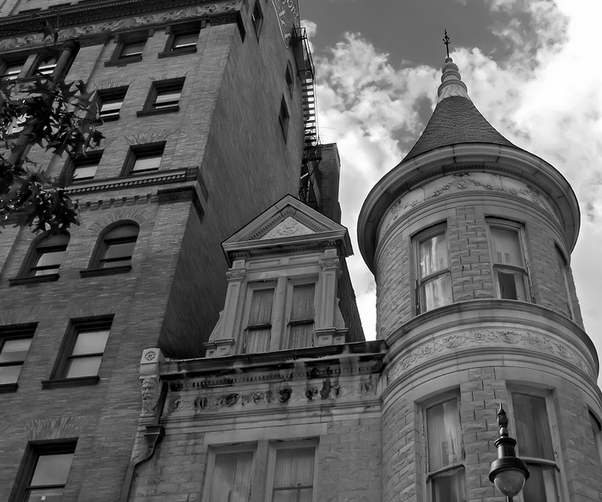
\includegraphics[width=.9\textwidth]{backgroundTheory/segmentation/Building} \\
(a)
\end{tabular}
\end{minipage}
\begin{minipage}{.45\textwidth}
\begin{tabular}{c}

\includegraphics[width=.9\textwidth]{backgroundTheory/segmentation/LoG} \\
(b)
\end{tabular}
\end{minipage}
\\
\begin{minipage}{.45\textwidth}
\begin{tabular}{c}

\includegraphics[width=.9\textwidth]{backgroundTheory/segmentation/sobelHorizontal} \\
(c)
\end{tabular}
\end{minipage}
\begin{minipage}{.45\textwidth}
\begin{tabular}{c}

\includegraphics[width=.9\textwidth]{backgroundTheory/segmentation/sobelVertical} \\
(d)
\end{tabular}
\end{minipage}
\caption{(a): Image to be segmented, (b): LoG, (c): Sobel - highlighting horizontal edges, (d):Sobel - highlighting vertical edges}
\label{edgeSeg}
\end{figure}

\subsubsection{Canny edge detector}
A more powerful edge detection method is the Canny edge detector. This method consist of four steps. The first step is to smooth the image based on a Gaussian filter with a given standard deviation \(\sigma\). In the next step the derivatives in both directions are computed using any first order operator, and using these the gradient magnitude image and its direction are computed. The gradient magnitude image typically contains wide ridges around local maxima of the gradient. In order to get a single response to an edge, only local maxima should be marked as edges, and this process is called non-maxima suppression. A simple way for non-maxima suppression is to first quantize the edge directions according to 8-connectivity (or 4 connectivity). Then consider each pixel with magnitude \(> 0\) as candidate edge pixels. For every candidate edge pixel look at the two neighboring pixels in edge-direction and the opposite direction. If the magnitude of the candidate edge pixel is not larger than the magnitude of these neighboring pixels, mark the pixel for deletion. When all candidate edge pixels are inspected, remove all the candidates that are marked for deletion. Now all the edges will contain a single response, but there still are lines/pixels that are not part of any continues edge. To remove these, hysteresis thresholding is used. Hysteresis thresholding consist of segmenting the image with two threshold values. First, the non-maxima supressed images is thresolded with a high thresold value \(T_h\) that determines which of the remaining candidate edge pixels are immediately considered as edge pixels (strong edges). The high threshold value leads to an image with broken edge contours. Therefore a low thresold value \(T_l\) is used to threshold the non-maxima supressed image again. The pixels in this segmented image that are connected to a strong edge are added to the final edge image.

The Canny edge detector gives different results based on the values of \(\sigma\), \(T_h\) and \(T_l\), but the derivative operator used to find the magnitude and how the non-maxima suppression was implemented also affects the final edge segmented image.

\section{Level Set Method}
\label{levelSetChap}
\subsection{Introduction}
Surfaces that evolves over time can be difficult to represent. Taking the surface in figure \ref{interface} as an example, assume that the red surface is heat and the arrows on the interface as the direction of its movement, which is normal to the interface itself. One way to represent the propagation of this interface is by the function $y = f(x,t)$, where $t$ represents time and $x,y$ are coordinates. The problem with this representation is that it cannot represent every concievable shape of the interface. If for instance the shape
of the interface has more y coordinates for a particular x coordinate (which is true for all closed interfaces), the interface cannot be correctly represented using this notion.
\begin{figure}[h!]
\centering
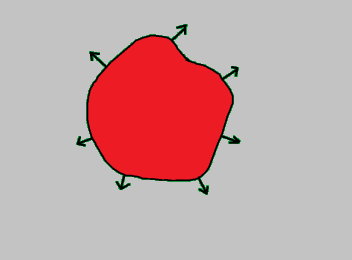
\includegraphics[width=.5\textwidth]{backgroundTheory/levelset/interface}
\caption{Interface of a moving surface.}
\label{interface}
\end{figure}
A better alternative is to use a parametric equation. The problem mentioned above would then be solved because the interface would only depend on the time variable t. But parametric representation of evolving interfaces have its own difficulties. When a surface evolves, the model have to be reparemeterized, which, due to the computional overhead (especially in 3D) add limitations to what kind of shapes a parameterical model can represent effectively. Topological changes, such as splitting or merging parts during the propagation is difficult to represent using parametric models. Sharp corners, distant edges blending together and the complexity of representing boundaries in higher dimensions are some other reasons why an evolving surface is difficult to represent parametrically. A simple example is shown in figure \ref{problematicEvo}, the two interfaces have to be represented as a single parametric function when merging and as two seperate againg when they split, and some sort of collison detection must be used to discover when the interfaces merge/split.
\begin{figure}[h!]
\centering
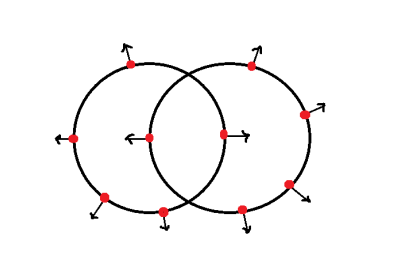
\includegraphics[width=.5\textwidth]{backgroundTheory/levelset/twoCircles}
\caption{Interface evolution difficult to represent parametrically.}
\label{problematicEvo}
\end{figure}

As a solution to all the problems mentioned above Osher and Sethian introduced the level set method in 1988 in \cite{osher88}. The main idea behind the level set method is to represent the interface of a surface implicitly by using a higher dimensional function. Adding an extra dimension simplifies the problems mentioned above significantly. This higher dimension function is called the level set function, and a 2D interface (a curve) is represented by the 3D level set function
\begin{equation}
\phi(x, y, t) 
\end{equation}
where the additional dimension \(t\) represents time. Similarly any 3D or higher level function can be represented by a level set function by adding one dimension. At a given time step, the evolving surface/model can be represented as a closed curve by the boundary of the level set at that time step. This representation of the model is called the zero level set and is defined as the set of points where the level set is zero:
\begin{equation}
\Gamma(x, y, t) = \{\phi(x, y, t) = 0\}. 
\end{equation}
The initial curve is at the xy-plane, that is, at \(\phi(x,y,0)\). As an example, figure \ref{levelsetEx}a depicts a circle with arrows pointing in the direction it is evolving, and figure \ref{levelsetEx}b is the cone that represents the corresponding level set function with the start-position in red.

\begin{figure}[h!]
\centering
\begin{minipage}{.4\textwidth}
\begin{tabular}{c}
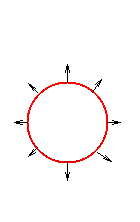
\includegraphics[height=.3\textheight]{backgroundTheory/levelset/f1a} \\
(a)
\end{tabular}
\end{minipage}
\begin{minipage}{.4\textwidth}
\begin{tabular}{c}
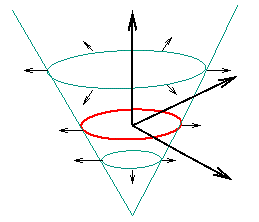
\includegraphics[height=.3\textheight]{backgroundTheory/levelset/f1b} \\
(b)
\end{tabular}
\end{minipage}
\caption{(a): Circle with arrows pointing in direction of movement, (b): Corresponding level set function}
\label{levelsetEx}
\end{figure}

Assuming that the zero level set moves in a direction normal to the speed F, then \(\phi\) satisfies the level set equation
\begin{equation}
\frac{\partial \phi}{\partial t} = |\nabla \phi|F
\label{levelSetEq}
\end{equation}
which is used to update the level set at each time step (iteration). Here \(|\nabla \phi|\) represents the gradient of \(\phi\), and the speed function F describes how each point in the boundary of the surface evolves. The level set method is applied in many different contexts, such as image processing, fluid dynamics and other simulations, and the speed function F depends on the type of problem being considered. 

An often used speed function for image segmentation that combines a data term and the mean curvature of the surface is \cite{cates03,lefohn04}
\begin{equation}
F = \alpha D(I) + (1-\alpha) \nabla \frac{\nabla \phi}{|\nabla \phi|}
\end{equation} 
where \(\nabla \cdot (\nabla \phi / |\nabla \phi|)\) is the normal vector that represents the mean curvature term which keeps the level set function smooth. \(D(I)\) is the data function that forces the model towards desirable features in the input data. The free weighting parameter \(\alpha \in{[0,1]}\) controls the level of smoothness, and I is the input data (the image to be segmented). The smoothing term \(\alpha\) restricts how much the curve can bend and thus alleviates the effect of noise in the data, preventing the model from leaking into unwanted areas\cite{lefohn04}. This is one of the big advantages the level set method has over classical flood fill, region grow and similar algorithms, which does not have a constraint on the smoothness of the curve.

A simple data function for any point (pixel, voxel) based solely on the input intensity I at that point\cite{cates03,lefohn04} is:
\begin{equation}
D(I) = \epsilon - |I - T|
\end{equation} 
Here \(T\) is the central intensity value of the region to be segmented, and \(\epsilon\) is the deviation around \(T\) that should also considered to be inside the region. This makes the model expand if the intensity of the points are within the region \(T \pm \epsilon\), and contract otherwise. The data function is gradual, thus the effects of \(D(I)\) diminish as the model approaches the boundaries of regions with gray-scale levels within the \(T \pm \epsilon\) range \cite{lefohn04}. This results in the model expanding faster with higher values of \(\epsilon\) and slower with lower values. 

The level set algorithm is initialized by placing a set of seed points that represents a part inside the region to be segmented. These seed points are represented by a binary mask of the same size as the image to be segmented. This mask is used to compute the signed distance function which \(\phi\) will be initialized to. 

\subsection{Signed Distance Transform}
A distance function \(D: \mathbb{R}^3 \rightarrow \mathbb{R}\) for a set S is defined as 
\begin{equation}
D(r,S) = min(r-S) \quad for \ all \ r \in{\mathbb{R}^3}
\end{equation}
If a binary image have one or more objects, a distance function can be used to assign a value for every pixel (or voxel in 3D) that represents the minimum distance from that pixel to the closest pixel in the boundary of the object(s). That is, the pixels in the boundary of an object are zero valued, and all other pixels represent the distance to the boundary as a value. Using a distance transform was the idea of how to initialize \(\phi\) in \cite{osher88}, where it was initialized as \(\phi = 1 \pm D^2\). But in \cite{mulder92} it was showed that initializing \(\phi\) to a signed distance function gives more accurate results. Signed distance transforms (SDT) assign for each pixel a value with a positive or negative sign that depend on whether the pixel is inside or outside the object. The values are usually set to be negative for pixels that are inside an object, and positive for those outside. The pixels of the model, which represents the boundary (the zero level set), have values 0. A binary image containing an object is shown in figure \ref{SDT}a (the numbers in this image represent intensity values). Figure \ref{SDT}b is the signed distance transform of \ref{SDT}a where city-block (manhattan) distance have been used, and figure \ref{SDT}c is the signed Euclidean distance transform (SEDT).

\begin{figure}[h!]
\centering
\begin{minipage}{.45\textwidth}
\begin{tabular}{c}
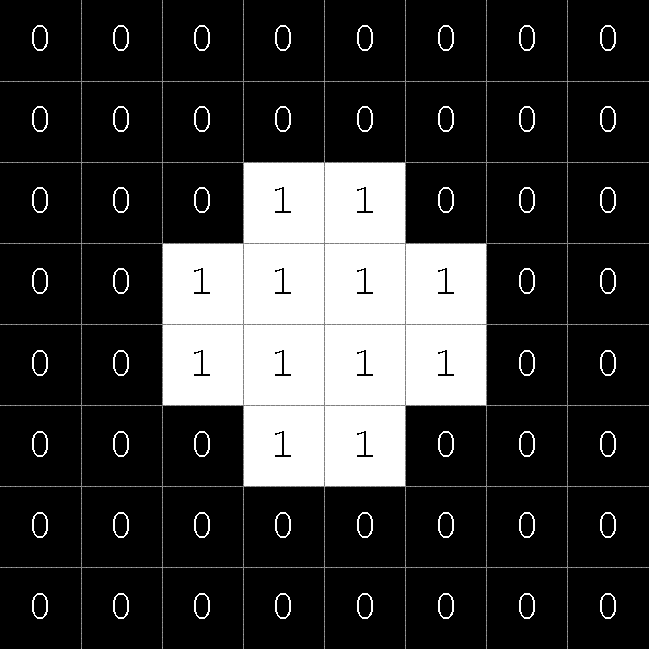
\includegraphics[width=.9\textwidth]{backgroundTheory/levelset/orgNew} \\
(a)
\end{tabular}
\end{minipage}
\begin{minipage}{.45\textwidth}
\begin{tabular}{c}
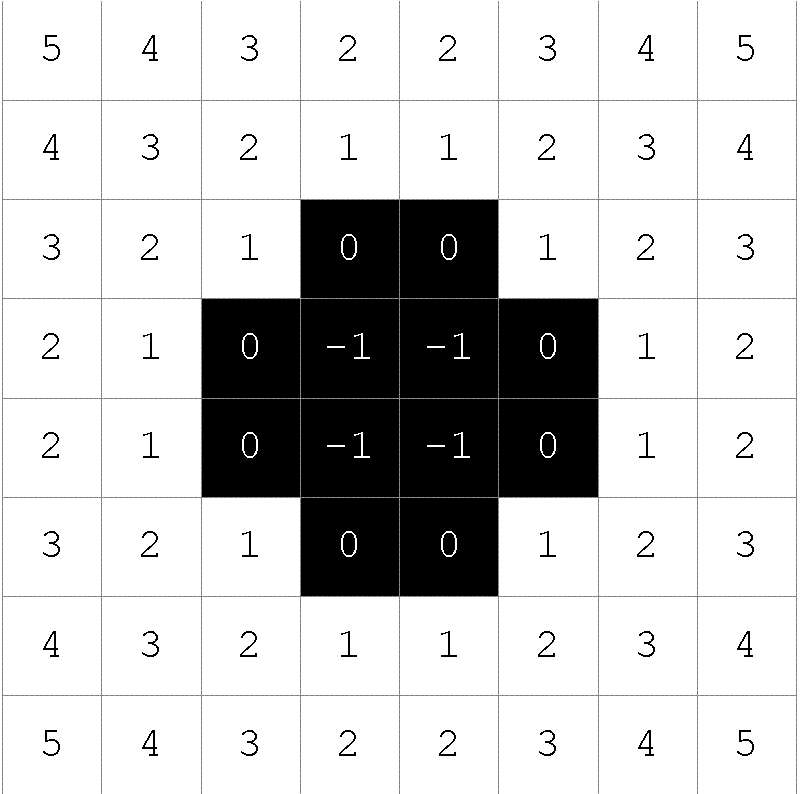
\includegraphics[width=.9\textwidth]{backgroundTheory/levelset/manhattan} \\
(b)
\end{tabular}
\end{minipage}
\\
\begin{tabular}{c}
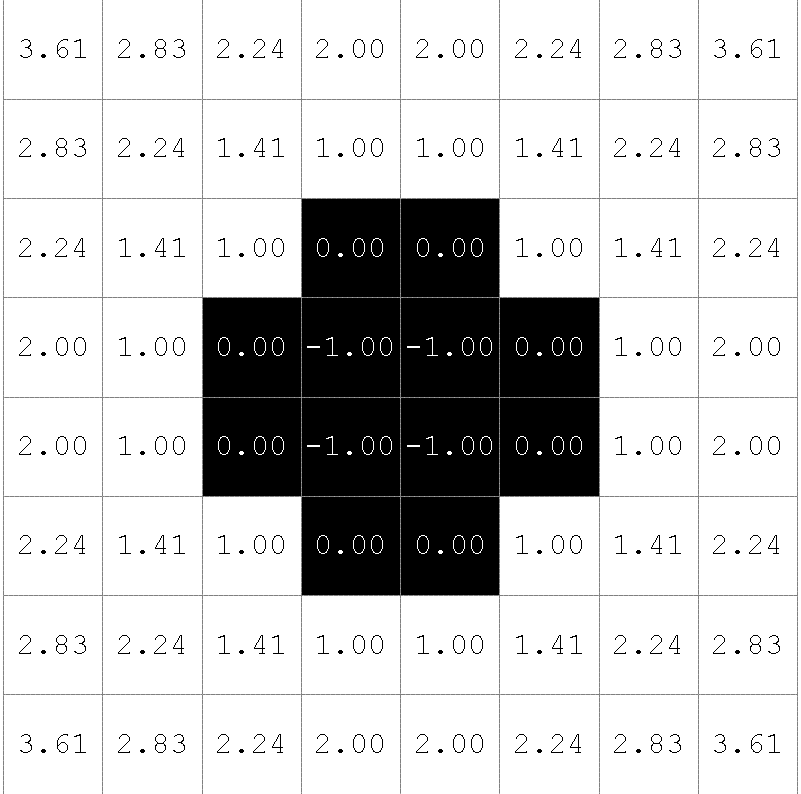
\includegraphics[width=.5\textwidth]{backgroundTheory/levelset/euclidean} \\
(c)
\end{tabular}
\caption{(a): Binary image, (b): SDT based on city-block distance, (c): SDT based on euclidean distance}
\label{SDT}
\end{figure}

As can be seen from the figures above, using different kind of functions for the SDT can result in different distances. These differences effects the accuracy of the level set function, which may leads to different end-results of the segmentation, hence, the function used to represent the distance have to be carfully chosen. However, sometimes a less accurate SDT have to be used as a tradeoff for faster computation time.

%\subsection{Sparse Field}
%The narrow band  method assumes that the computation of the SDT is so slow that it cannot be computed for every iteration (time step). The sparse field method introduced in \cite{whitaker89} uses a fast approximation of the distance transform that makes it feasible to compute the neighborhood of the level set model for each iteration. In the sparse field method the idea of using a thin band is taken to the extreme by working on a band that is only one point wide. The points adjacent to the level set are called active points, and all of them together are referred to as the active set. At each iteration only a thin layer of points near the active set are visited and updated. Using only the active points to compute the derivatives would not give sufficient accuracy. Because of this, the method extends out from the active points in small layers to create a neighborhood that is precisely the width needed to calculate the derivatives needed. 

%Several advantages to this approach are mentioned in \cite{whitaker89}. No more than the precise number of calculations to find the next position of the zero level set surface is used. The number of points being computed is so small that a linked-list can be used to keep track of them. This also results in that only those points whose values control the position of the zero level set surface are visited at each iteration. A disadvantage of the narrow band method is that the stability at the boundaries of the band have to be maintained (e.g. by smoothing) since some points are undergoing the evolution while other neighbouring points remain fixed. The sparse field method avoid this by not letting any point entering or leaving the active set affecting its value. A point enters the active set if it is adjacent to the model. As the model evolves, points in the active set that are no longer adjacent to the model are removed from the active set. This is done by defining the neighborhoods of the active set in layers and keeping the values of points entering or leaving the active set unchanged. A layer is a set of pixels represented as \(L_{i}\) where \(i\) is the city-block distance from the active set. The layer \(L_{0}\) represents the active set, and \(L_{\pm 1}\) reprsents pixels adjacent to the active set on both sides. Using linked lists to represents the layers and arrays (matrices) to represent distance values makes the algorithm very efficient. The exact steps of the sparse field algorithm can be found in \cite{whitaker89}.

%The sparse field algorithm is based on an important approximation, it assumes that points adjacent to the active points undergoes the same change in value as their nearby active set neighbors. But despite this, the errors introduced by the sparse field algorithm are no worse than many other level set algorithms. Since only those grid points whose values are changing (the active points and their neighbors) are visited at each time step the growth computation time is \(d^{n-1}\), where d is the number of pixels in along one dimension of the image. This is the same as for parameterized models where the computation times increase with the resolution of the domain, rather than the range.

\subsection{Discretization by upwinding and difference of normals}
\label{upwinding}
To use the level set method in image processing it have to be discretized, but simple forward finite difference schemes cannot be used because such schemes tends to overshoot and are unstable. To overcome this problem the up-winding scheme was proposed in \cite{osher88}. To avoid the overshooting problems associated with forward finite differences the up-winding scheme uses one-sided derivatives that looks in the up-wind direction of the moving interface. Let \(\phi^n\) and \(F^n\) represent the values of \(\phi\) and \(F\) at some point in time \(t^n\). The updating process consist of finding new values for \(\phi\) at each point after a time interval \(\Delta t\). The forward Euler method is used to get a first-order accurate method for the time discretization of equation \ref{levelSetEq}, given by (from \cite{osher02})
\begin{equation}
\frac{\phi^{n+1}-\phi^n}{\Delta t} + F^n \cdot \nabla \phi^n = 0
\label{discEq}
\end{equation}
where \(\phi^{n+1}\) is \(\phi\) at time \(t^{n+1} = t^n + \Delta t\), and \(\nabla \phi^n\) is the gradient at time \(t^n\). This equation is expanded as follows (for three dimensions):
\begin{equation}
\frac{\phi^{n+1}-\phi^n}{\Delta t} + u^n \phi_x^n + v^n \phi_y^n + w^n \phi_z^n= 0,
\label{discEqExpanded}
\end{equation}
where the techniques used to approximate the \(u^n \phi_x^n\), \(v^n \phi_y^n \) and \(w^n \phi_z^n\) terms can be applied independently in a dimension-by-dimension manner \cite{osher02}. When looking at only one dimension (for simplicity), the sign of \(u^n\) would indicate whether the values of \(\phi\) are moving to the right or to the left. The value \(u^n\) can be spatially varying, hence by looking at only one point \(x_i\) in addition to only look at one dimension, equation \ref{discEqExpanded} can be written as
\begin{equation}
\frac{\phi_i^{n+1}-\phi_i^n}{\Delta t} + u_i^n (\phi_x)_i^n = 0,
\label{discEq1DPoint}
\end{equation}  
where \((\phi_x)_i^n\) denotes the spatial derivative of \(\phi\) at point \(x_i\) at time \(t^n\). The values of \(\phi\) are moving from left to right if \(u_i > 0\), thus the points to the left for \(x_i\) are used to determine the value of \(\phi\) at point \(x_i\) for the the next time step. Similarly, if \(u_i < 0\) the movement is from right to left, and the points to the right of \(x_i\) are used. As a result, \(\phi_x\) is approximated by the derivative function \(D_x^+\) when \(u_i < 0\) and \(D_x^-\) when \(u_i > 0\). When \(u_i = 0\) the term \(u_i(\phi_x)_i\) equals zero, and approximation is not needed. Extending this to three dimensions, the derivatives used to update the level set equation are 
\begin{equation*}
\nonumber D_x = \frac{\phi_{i+1,j,k} - \phi_{i-1,j,k}}{2} \quad D_y = \frac{\phi_{i,j+1,k}-\phi_{i,j-1,k}}{2} \quad D_z = \frac{\phi_{i,j,k+1}-\phi_{i,j,k-1}}{2} 
\end{equation*}
\begin{equation*}
\nonumber D_x^+ = \phi_{i+1,j,k} - \phi_{i,j,k} \quad D_y^+ = \phi_{i,j+1,k} - \phi_{i,j,k} \quad D_z^+ = \phi_{i,j,k+1} - \phi_{i,j,k} 
\end{equation*}
\begin{equation*} 
D_x^- = \phi_{i,j,k} - \phi_{i-1,j,k} \quad D_y^+ = \phi_{i,j,k} - \phi_{i,j-1,k} \quad D_z^+ = \phi_{i,j,k} - \phi_{i,j,k-1}
\end{equation*}
\begin{equation}
\quad %to get a reference number below the equations
\end{equation}
which is taken from the appendix of \cite{lefohn04}. This is a \textit{consistent} finite difference approximation to the level set equation in \ref{levelSetEq}, because the approximation error converges to zero as \(\Delta t \rightarrow 0\) and \(\Delta x \rightarrow 0\) \cite{osher02}. In addition to being consistent, it also have to be \textit{stable} in order to get the correct solution. Stability guarantees that small errors in the approximations are not amplified over time. The stability can be enforced using the  Courant-Friedreichs-Lewy (CLF) condition which says that the numerical wave speed \(\frac{\Delta x}{\Delta t}\) must be greater than the physical wave speed \(|u|\),
\begin{equation}
\Delta t = \frac{\Delta x}{max\{|u|\}},
\end{equation}
where \(max\{|u|\}\) is the largest value of \(|u|\) on the model.

The gradient \(\nabla \phi\) is approximated to either \(\nabla \phi_{max}\) or \(\nabla \phi_{min}\) depending on whether the speed function for a given point \(F_{i,j,k}\) is positive or negative, 
\begin{equation}
\nabla \phi = \left\{
\begin{array}{l l}
||\nabla \phi_{max}||_2 & F_{i,j,k}>0 \\
||\nabla \phi_{min}||_2 & F_{i,j,k}<0
\end{array} \right.
\end{equation}
where \(\nabla \phi_{max}\) and \(\nabla \phi_{min}\) is given by (from \cite{lefohn04})
\begin{equation}
\nabla \phi_{max} = \begin{bmatrix}
\: \sqrt{max(D_x^+,0)^2 + max(-D_x^-,0)^2} \: \\[1.5em]
\: \sqrt{max(D_y^+,0)^2 + max(-D_y^-,0)^2} \: \\[1.5em]
\: \sqrt{max(D_z^+,0)^2 + max(-D_z^-,0)^2} \: 
\end{bmatrix} 
\end{equation}
\newline
\begin{equation}
\nabla \phi_{min} = \begin{bmatrix}
\: \sqrt{min(D_x^+,0)^2 + min(-D_x^-,0)^2} \: \\[1.5em]
\: \sqrt{min(D_y^+,0)^2 + min(-D_y^-,0)^2} \: \\[1.5em]
\: \sqrt{min(D_z^+,0)^2 + min(-D_z^-,0)^2} \: 
\end{bmatrix} 
\end{equation}

The curvature term \(\nabla \cdot (\nabla \phi / |\nabla \phi|)\) of the speed function \(F\) is discretized using the difference of normals method. The second order derivatives are computed first:
\begin{equation*}
D_x^{+y} = (\phi_{i+1,j+1,k} - \phi_{i-1,j+1,k})/2 \quad D_x^{-y} = (\phi_{i+1,j-1,k} - \phi_{i-1,j-1,k})/2 
\end{equation*}
\begin{equation*}
D_x^{+z} = (\phi_{i+1,j,k+1} - \phi_{i-1,j,k+1})/2 \quad D_x^{-z} = (\phi_{i+1,j,k-1} - \phi_{i-1,j,k-1})/2 
\end{equation*}
\begin{equation*}
D_y^{+x} = (\phi_{i+1,j+1,k} - \phi_{i+1,j-1,k})/2 \quad D_y^{-x} = (\phi_{i-1,j+1,k} - \phi_{i-1,j-1,k})/2 
\end{equation*}
\begin{equation*}
D_y^{+z} = (\phi_{i,j+1,k+1} - \phi_{i,j-1,k+1})/2 \quad D_y^{-z} = (\phi_{i,j+1,k-1} - \phi_{i,j-1,k-1})/2 
\end{equation*}
\begin{equation*}
D_z^{+x} = (\phi_{i+1,j,k+1} - \phi_{i+1,j,k-1})/2 \quad D_z^{-x} = (\phi_{i-1,j,k+1} - \phi_{i-1,j,k-1})/2 
\end{equation*}
\begin{equation*}
D_z^{+y} = (\phi_{i,j+1,k+1} - \phi_{i,j+1,k-1})/2 \quad D_z^{-y} = (\phi_{i,j-1,k+1} - \phi_{i,j-1,k-1})/2 
\end{equation*}
\begin{equation}
\quad %to get a reference number below the equations
\end{equation}
Then these derivatives are used to compute the normals \(n^+\) and \(n^-\) in equation \ref{normals}, which is used to compute the mean curvature \(H\) in equation \ref{meanCurvature} taken from \cite{lefohn04}.
\begin{equation*}
n^+ = \begin{bmatrix}
\: \frac{D_x^+}{\sqrt{(D_x^+)^2 + (\frac{D_y^{+x}+D_y}{2})^2 + (\frac{D_z^{+x}+D_z}{2})^2}} \: \\[2.5em]
\: \frac{D_y^+}{\sqrt{(D_y^+)^2 + (\frac{D_x^{+y}+D_x}{2})^2 + (\frac{D_z^{+y}+D_z}{2})^2}} \: \\[2.5em]
\: \frac{D_z^+}{\sqrt{(D_z^+)^2 + (\frac{D_x^{+z}+D_x}{2})^2 + (\frac{D_y^{+z}+D_y}{2})^2}} \:
\end{bmatrix} 
\end{equation*}
\begin{equation}
n^- = \begin{bmatrix}
\: \frac{D_x^-}{\sqrt{(D_x^-)^2 + (\frac{D_y^{-x}+D_y}{2})^2 + (\frac{D_z^{-x}+D_z}{2})^2}} \: \\[2.5em]
\: \frac{D_y^-}{\sqrt{(D_y^-)^2 + (\frac{D_x^{-y}+D_x}{2})^2 + (\frac{D_z^{-y}+D_z}{2})^2}} \: \\[2.5em]
\: \frac{D_z^-}{\sqrt{(D_z^-)^2 + (\frac{D_x^{-z}+D_x}{2})^2 + (\frac{D_y^{-z}+D_y}{2})^2}} \:
\end{bmatrix} 
\label{normals}
\end{equation}

\begin{equation}
H = \frac{1}{2}\nabla \cdot \frac{\nabla \phi}{|\nabla \phi|} = \frac{1}{2}[(n_x^+ - n_x^-) + (n_y^+ - n_y^-) + (n_z^+ - n_z^-)]
\label{meanCurvature}
\end{equation}

Finally, the level set equation is updated as
\begin{equation}
\phi(t + \Delta t) = \phi(t) + \Delta tF|\nabla \phi|.
\end{equation}
\section{Narrow Band - for lite?}
\subsection{Introduction}
When working with the level set of a single interface a huge drawback with the originally proposed level set method is the computional inefficiency due to computing over the whole domain of \(\phi\). As a solution to this problem Adalstein and Sethian proposed the narrow band method in 1994\cite{adalsteinsson94}. The narrow band looks at the interface of a single level set instead of the whole domain, and thereby decreases the computational labor of the standard level set method for propagating interfaces considerably. Another reason the narrow band was proposed are problems where the velocity field is only given on the interface. In such cases the construction of an appropriate speed funcion for the entire domain made use of the classical level set method a significant modeling problem.

\subsection{Overview of the Narrow Band method}
Unlike the original level set method, which describe the evolution of an embedded family of contours, the narrow band works with only a single surface model\cite{whitaker89}. That is, instead if calculating $\phi$ over the whole domain it focuses only on a small part surrounding the surface. There are many cases in which the description of the evolution of only one surface in the domain is needed, and in such cases the narrow band method operates much faster while delivering the same results. The method ignores points that are far away from the zero level set at each iteration and only looks at the points within a narrow band. This is possible because points far away from the zero level set do not have any influence on the result. That is, only the area of $\phi$ where \(\phi \approx 0\) is important for accurate representation of the level set. The narrow band method restrict the computation to a thin band of points by extending out approximately k points from the zero level set (shown in figure \ref{narrowBand}), and an embedding of the evolving interface is constructed via a signed distance transform. All points outside the band is set to constant values to indicate that they are not within the band and thus should not be used in the computation. This reduces the number of operations at each iteration from \(O(n^{d+1})\) to \(O(nk^{d})\) \cite{adalsteinsson94} where d is the number of dimensions and n is the (average) number of points in one dimension. 
\begin{figure}[h!]
\centering
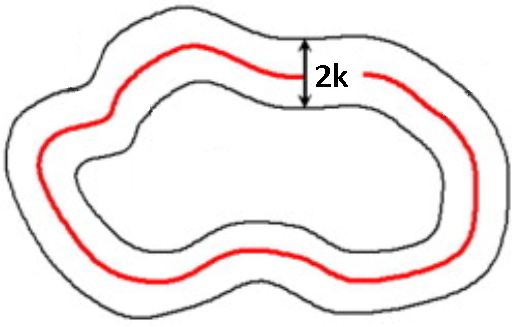
\includegraphics[width=.5\textwidth]{backgroundTheory/levelset/narrowBand}
\caption{The narrow band extending out with a width of k from the level set.}
\label{narrowBand}
\end{figure}
The points within the band is used to calculate the distance function and then to initialize $\phi$ to the signed distance. As the zero level set evolves, \(\phi\) will get further and further away from its initialized value as signed distance. As this happens \(\phi\) must be ensured to stay within the band. One way to do this would be to make a new band for each iteration. But determining which points are to be inside the band, and deciding how to take the differentials at the edge points makes the reconstruction process of the band time consuming. Thus a given band is used for several iterarions with the same initialization of \(\phi\). When the interface gets close to the band it has to be reset from the current position of the zero level set and \(\phi\) must be reinitialized. Reinitializing \(\phi\) at every iteration takes too much time and the alternative task of finding out if any of the pixels in the zero level set are getting close to the edge of the band (for every iteration) also takes time. Hence, \(\phi\) is usually just reinitialized after a fixed number of iterations, which keeps \(\phi\) approximately equal to the SDT. 

As metioned in the section about signed distance transforms, different SDTs can lead to slightly different end-results and must be carefully chosen. If the technique used to approximate \(\phi\) to a signed distance function is too sensitive, \(\phi\) needs to be reinitialized accurately and often. If it is less sensitive, it does not have to be initialized so often and a less accurate method can be used, but this may lead to noisy features \cite{osher02}.

The narrow band, despite its improvements over the original level set method, is not optimal. The band used being too wide is the main reason. Even if k=2 is enough to compute the necessary derivatives, the band have to be of a certain width (k=12 was used in the test of topological changes in \cite{adalsteinsson94}) because of two competing computional costs\cite{whitaker89}. The first is the cost of computing the position of the curve and the SDT, and reset the band. The second is the cost of computing the evolution process over the entire band.

\chapter{Sparse Field}

\section{Theory} //Theory eller introduction som seksjons-overskrift?

The narrow band  method assumes that the computation of the SDT is so slow that it cannot be computed for every iteration. The sparse field method introduced in \cite{whitaker89} uses a fast approximation of the distance transform that makes it feasible to compute the neighborhood of the level set model for each iteration. In the sparse field method the idea of using a thin band is taken to the extreme by working on a band that is only one point wide. The points (immediately?) adjacent to the level set are called active points, and all of them together are referred to as the active set. At each iteration only a thin layer of points near the active set are visited and updated. Using only the active points to compute the derivatives would not give sufficient accuracy. Because of this, the method extends out from the active points in small layers to create a neighborhood that is precisely the width needed to calculate the derivatives needed. 

Several advantages to this approach are mentioned in \cite{whitaker89}. No more than the precise number of calculations to find the next position of the zero level set surface is used. The number of points being computed is so small that a linked-list can be used to keep track of them. This also results in that only those points whose values control the position of the zero level set surface are visited at each iteration. 


A disadvantage of the narrow band method is that the stability at the boundaries of the band have to be maintained (e.g. by smoothing) since some points are undergoing the evolution while other neighbouring points remain fixed. The sparse field method avoid this by not letting any point entering or leaving the active set affecting its value. A point enters the active set if it is adjacent to the model. As the model evolves, points in the active set that are no longer adjacent to the model are removed from the active set. This is done by defining the neighborhoods of the active set in layers and keeping the values of points entering or leaving the active set unchanged. A layer is a set of pixels represented as \(L_{i}\) where \(i\) is the city-block distance from the active set. The layer \(L_{0}\) represents the active set, and \(L_{\pm 1}\) reprsents pixels adjacent to the active set on both sides. Using linked lists to represents the layers and arrays (matrices) to represent distance values makes the algorithm very efficient. 

The sparse field algorithm is based on an important approximation, it assumes that points adjacent to the active points undergoes the same change in value as their nearby active set neighbors. But despite this, the errors introduced by the sparse field algorithm are no worse than many other level set algorithms. Since only those grid points whose values are changing (the active points and their neighbors) are visited at each time step the growth computation time is \(d^{n-1}\), where d is the number of pixels in along one dimension of the image. This is the same as for parameterized models where the computation times increase with the resolution of the domain, rather than the range. 



The Up-Winding scheme gives the curvature in an area surrounding a point in the active set. This scheme uses both first and second order derivatives, and to calculte them it needs a 3x3x3(3D) grid of points surrounding the point for which it is calculating the speed. 


\section{Implementation}

We implemented the Sparse Field method using C/C++. Out implementation used lists, a C++ struct, to maintain the different




Cutouts and working progress stuff:

The neighbours of the active set are tracked in lists, L1, L2, L-1 and L-2, and in addition we have the active set L0. These lists keep track of the coordinates of where the different layers reside in each iteration. 






\chapter{Sparse Field - Implemented code}
\section{Introduction}
The sparse field level set method was implemented in C++ for the project, and the implemented code is mainly based on the pseudocode in \cite{lankton09}, which again is based on Whitaker's introduction to the sparse field method in \cite{whitaker89}. 
The sparse field was first implemented in 2D and after bugfixing and some test-runs it was extended to 3D, which is executed in the exact same was as the 2D version. Both the 2D and 3D versions of the implemented code can be found in appendix B, and the pseudocode (only in 2D) can be found in appendix A. In this chapter the pseudocode in \cite{lankton09} will be explained first, along with how it works. Secondly, the differences between Lankton's pseudocodes in \cite{lankton09} and the implemented code will be described. And finally there will be a detailed explanation of the implemented code.

\section{TODO}
As previously mentioned, the sparse field method can be implemented using linked lists to hold the pixels being used in the calculations. Pixels in this context does not mean the pixels in the original or segmented image, but the points in the matrix that represents the $\phi$. These pixels are seperated into five layers, each represented by a linked list. One of the lists holds the active points, i.e the zero level set, and is referred to as the Lz list. The rest of the needed pixels are seperated according to their closeness to the pixels in Lz and which side of the Lz pixels they are located. The Ln1 list contains the pixels that are adjacent to Lz pixels on the inside of the object being segmented. Similarly Lp1 contains pixels that are adjacent, but on the outside. All pixels that are adjacent to those in Ln1 except for those in Lz are elements in the Ln2 list, and similarly the ones adjacent to Lp1 on the opposite side of Lz are part of Lp2. This becomes more clear when looking at table \ref{rangeTab1} and figure \ref{labelExample}. 

\begin{table}[h] %h = here
	\begin{tabular}{| c | c |} 
	% l = left-justified columns, alternatives are: r (right) and c (center)
	% | = vertical line, \hline = horizontal line
	\hline
	List Name & Range\\
	\hline
	Lz & [-0.5, 0.5]\\
	Ln1 & [-1.5, -0.5>\\
	Lp1 & <0.5, 1.5]\\
	Ln2 & [-2.5, -1.5>\\
	Lp2 & <1.5, 2.5]\\
	\hline
	\end{tabular}
	\caption{Range of lists used in \cite{lankton09}}
	\label{rangeTab1}
\end{table}

\begin{figure}[h!]
\centering

\includegraphics[width=0.65\textwidth]{implemented/labelExample}
\caption{Label image: image showing the different layers under segmentation.}
\label{labelExample}
\end{figure}

Figure \ref{labelExample} represents the 5 different layers with different colors. The black colored part is defined to be inside the object being segmented, the white part as outside, and these two parts are not used in the computation for the current iteration. The dark blue pixels around the dark part are the pixels contained in Ln2, and the brown pixels are those on Ln1. The dark-purple colored pixels are Lz elements, light-purple are Lp1 and light-blue are pixels in Lp2. This type of image will henceforth be referred to as the $label$ image, because it shows the labels of the image being segmented.

\section{Forskjeller fra vår kode og pseudokoden til lankton}
Some improvements and changes from Lankton's pseudocode were made
By looking closer at table \ref{rangeTab1} it can be seen that Lz has a slightly wider ramge than the other lists. This range of exactly 1 does in some cases cause huge problems that lead to disortions and artifacts in the segmentation. What these problems are will be discussed in \ref{ProblemsMet}. To overcome these problems the ranges of the lists were slightly changed to make all the lists equal in range. The range-corrected lists are shown in table \ref{rangeTab2}, and even though the change seems insignificant it actually does change the result significantly (as will be discussed in \ref{ProblemsMet}).

\begin{table}[h] %h = here
	\begin{tabular}{| c | c |} 
	% l = left-justified columns, alternatives are: r (right) and c (center)
	% | = vertical line, \hline = horizontal line
	\hline
	List name & Range\\
	\hline
	Lz & [-0.5, 0.5>\\
	Ln1 & [-1.5, -0.5>\\
	Lp1 & [0.5, 1.5>\\
	Ln2 & [-2.5, -1.5>\\
	Lp2 & [1.5, 2.5>\\
	\hline
	\end{tabular}
	\caption{Range of lists used in the implementation}
	\label{rangeTab2}
\end{table}

\section{Om koden vår}
\subsection{Datastructures and types used - elr noe lignende}
In addition to the five lists representing the as five layers, two arrays of equal size and dimension as the image to be segmented are used. One of them is the $label$ image described above, which is used to track where the pixels containing the different layers are on the domain. Given a pixel, to find out which layer (if any) that pixel is a member of, a simple lookup to the $label$ is enough. Another excellent feature of the $label$ array is that it can be used to verify that all the layers are correclty aligned and if there are any pixels of any layers that are poorly placed. The $label$ image can thus be used to find artifacts that might have resulted from code errors. An example of a $label$ image (zoomed in to be able to clearly see the artifacts) which clearly states that there is something wrong with how the layers are handled in the code is shown in figure \ref{labelFailedEx}. How the $label$ label image actually should have been is illustrated in figure \ref{labelOkEx}.

\begin{figure}[h!]
\centering

\includegraphics[width=0.90\textwidth]{implemented/labelFailedEx}
\caption{A label image with pixels in places they should not be.}
\label{labelFailedEx}
\end{figure}

\begin{figure}[h!]
\centering

\includegraphics[width=0.90\textwidth]{implemented/labelOkEx}
\caption{How the label image should have been.}
\label{labelOkEx}
\end{figure}

The other array used is the $\phi$ - array, which contains the actual $\phi$ values of each pixel in the domain. The range of the values is exactly the same as in the $label$ image, but while the $label$ image only contains integer values describing which layer a pixel is part of, the $\phi$ image contains the actual values (floating point numbers) of the level set. The images represented by the $label$ and $\phi$ arrays would thus be very similar (though small differences may be seen) when looking at, but they do have different tasks. The $label$ is as mentioned used as a lookup table, while the $\phi$ array determines which layer a pixel belongs to after its pixels have been updated with the speed function.

To correctly move pixels between the layers some temporary lists have to be used, one for each layer. By using these temporary lists, called Sn2, Sn1, Sz, Sp2 and Sp2, pixels are prevented from being moved more than 1 layer at a single iteration. Assume that pixel $A$ is in Ln1 and has two neighbours in Lz. These two neighbours will be updated by the speed function and may move out of Lz into either Ln1 or Lp1. If both these pixels are moved out of Lz, pixel $A$ will no longer have any neighbours in Lz and will in most cases be incorrectly moved to Ln2. This is only of of many possible mistakes that could happen when not using temporary lists, an another example is that a pixel could be moved to a list and then back to where it came from within the same iteration. Using temporary lists prevent such problems by adding the pixels that are to change layer into them, removing the pixels from the original lists, and finally when all temporary lists are filled with pixels to be moved and all the original lists have the pixels moving out of them removed, then the original lists are filled with those in the temporary lists. And then the temporary lists are emptied before the next iteration starts.


FLYTT dette vekk til et annet sted...................
Before explaining what this means, a brief look into how the pixels are pushed to and popped from the different lists is needed. First the speed function is calculated for each pixel in Lz (will be explained in more detail in LINK TIL DER SPEED FUNCTION BLIR FORKLART). Then the four remaining lists are updated, but not using the speed function as with the Lz pixels. Since Ln1 and Lp1 are defined to be neighbours to Lz on each side, and Lp2 and Ln2 as neighbour to Lp1 Ln1 respectively, there is no need to use computation time to calculate their speed function. They will follow Lz, e.g. if a pixel in Lz moves to the right, then its neighbours (in Ln1 and Lp1) at each side will also move a step to the right. Similarly Ln2 and Lp2 pixels will follwow Ln1 and Lp1 respectively. How this actually is implemented is described in LINK HER

\subsection{Code structure}
The code is seperated into two C++ files, main.cpp and update.cpp, and two corresponding header files. The update.cpp file consist of everything that happens at each iteration, this icnludes calculating the speed function, updating the $\phi$ - array with the speed, updating the $label$ array and update the lists. The main.cpp file consist of actions that are executed before and after the actual segmentation, such as initializing everything, handle input and reading/writing to/from the input image and segmentation result. 

\subsection{Input and initialization}
TODO skriv om input\\
An array of same size as $label$ and the $\phi$ - arrays is used to initialize $label$, the $\phi$ - array and Lz. This array, called init, is initialized to zero valued elements at start, and then filled with 1's given the x,y (and z in 3D) coordinates along with a radius given as input. These input values creates a circle (or sphere if 3D) of 1's in the init array that represents the seed points. Multiple coodrinates and radiuses can be given as input to create multiple seed points. Based on the values in init the two arrays $label$ and $\phi$ are initialized. All pixels in $label$ and $\phi$ corresponding with the ones in init with value 1 are set to -3 to indicate that they are inside the segmentation object. All other pixels in $label$ and $\phi$ are set to 3 indicating that they are outside the object. Then the corresponding pixels to all values in init that are 1 but have 0 valued neighbours are set to 0, indicating that they are part of the zero level set. Then these pixels are added to Lz as initial zero level set values. Then $Ln1$, $Lp1$, $Ln2$ and $Lp2$ are filled according to their definitions, and the $label$ and $\phi$ arrays are updated to refelct these changes. After these initializing actions are finished the segmentation process can start. 
The $\phi$ - array is initialized by the using the x,y (and z in 3D) coordinates along with the radius to create a circle. This circle is 

\subsection{Speed function explained}
Two different speed functions are implemented. These are seperatly implemented in their own methods, and a speed function is only referenced in one place in the code. This makes it easy to implement new speed functions, and to change between which of them to use when running the program. The speed function methods takes in as parameters the coordinates of the pixel to calculate the speed chnage on, and returns a value which then is added to the speed from the last iteration. The two speed functions are implemented are the one explained in chapter \label{levelSetChap} and a much more simple one based on the Chan-Vese energy. Simply put, the Chan-Vese energy ($E^{CV}$) is defined as 
\begin{equation}
E^{CV}(c_1,c_2,C) = \int_{inside(C)} (\mu (x,y) - c_1)^2 \, dx \, dy \, + \, \int_{outside(C)} (\mu (x,y) - c_2)^2 \, dx \, dy \, \cite{wang10} %\, = whitespace
\end{equation}
where $\mu$ is the image, and C is a closed segmentation curve which in this case is the curve defined by the zero level set. The constants $c_1$ and $c_2$ are the average greyscale intensity values inside and outside of C, respectively. Discretizing this energy function, and writing it as a pixelwise function gives
\begin{equation}
E^{CV}(x,y) = (\mu (x,y) - c_1)^2 - (\mu (x,y) - c_2)^2
\end{equation}
TODO forklar litt om hvordan denne speed funksjonen virker\\
New speed functions can be implemented and easily mergeed with the rest of the code, but an importatnt factor that must be remembered is that the value returned from the speed function must be in the range $<-1,1>$, because of the range of the layers. Another important factor is that the lists representing the layers must support equal sized range-width ($<1$) because the speed function is calculated the exact same way for all elements regardless of which layer it is a member of. \\
TODO: Husk å skrive om hvorfor vi clamper verdiene mellom -1 og 1, istedenfor å normalisere (altså bare dele alt på dn høyeste mulige returnverdien)

\section{Problems met}
\label{ProblemsMet}
As previously mentioned, when looking at figure \ref{labelFailedEx} it can be clearly seen that something is wrong with how the lists (the layers) are arranged. This becomes even more clear when looking at figure \ref{failedZeroEx} which shows only the zero level set.
\begin{figure}[h!]
\centering
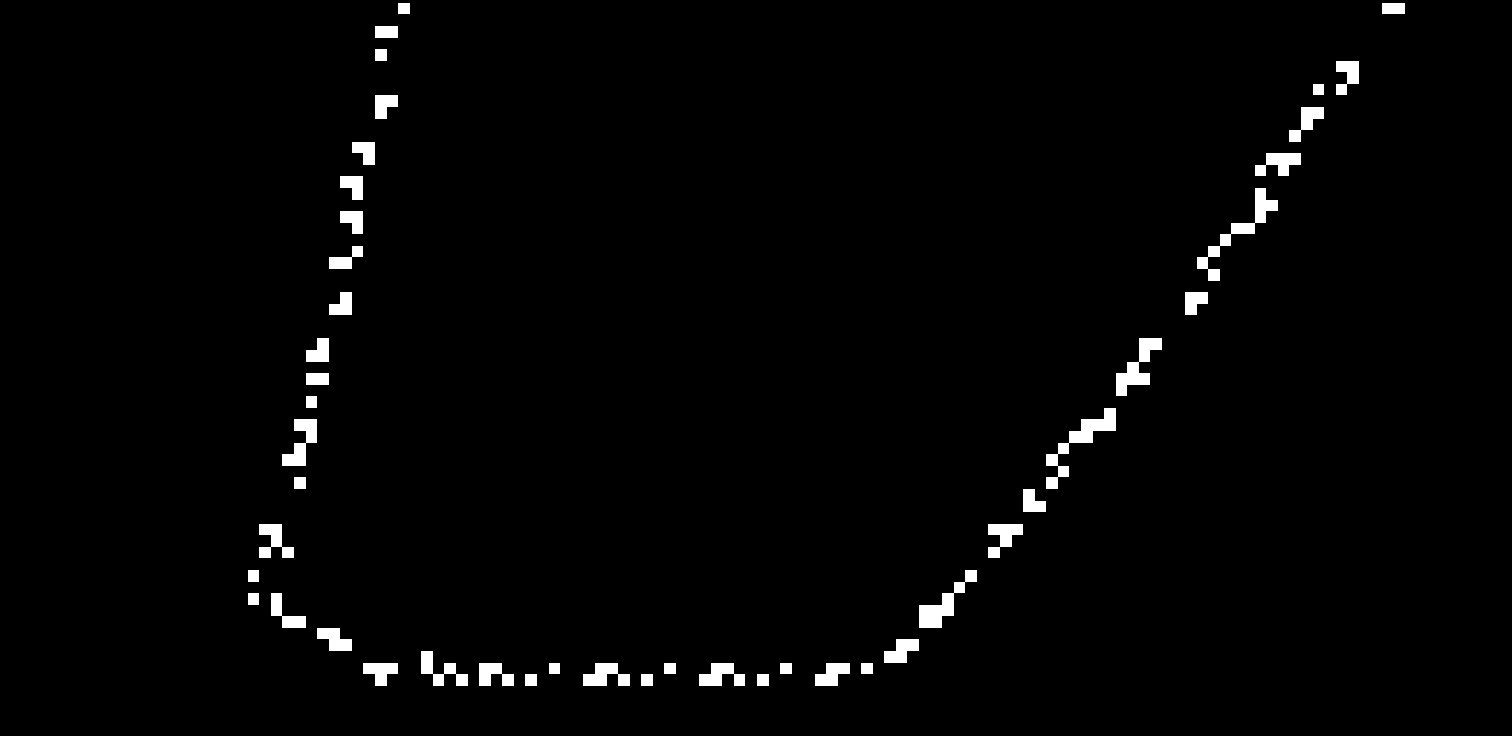
\includegraphics[width=0.90\textwidth]{implemented/failedZeroEx}
\caption{Zero level set corresponding to the label image in figure \ref{labelFailedEx}.}
\label{failedZeroEx}
\end{figure}
The zero level set in figure \ref{failedZeroEx} is the segmentation result (zoomed in) that corresponds to the label image in figure \ref{labelFailedEx}. The zero level set is supposed to be a one pixel wide continous line, but in this case that is not true. Several problems and bugs in the code combined were reasons were for this result. Much time and effort was used to debug this and to fix these problems. In addition to creating artifacts in the results, the bugs also made the program run much slower which made the debugging process even more time consuming. The main problem was that the layers were not of equal range-width and that the speed function was not normalized to be within the range $<\!-1,1\!>$, which will now be explained in more detail.
When an element in any of the five layers is updated by the speed function the new value may not reflect the range at which is allowed for the layer it is part of. In that case it have to be moved to another layer or in case the value is not in the allowed range of any of the layers removed from its current layer and not added to any other. The problem caused by the value returned by the speed function not being normalized was that elements in any layer was able to be transferred from its previous layer to a layer that is not a neihbouring layer. For example, transferring a pixel from Ln1 is restricted to the neighbouring layers of Ln1, namely Ln2 and Lz. But if a pixel $A$ in Ln1 with value -0.65 had its value increased by 1.2, its new value of 0.55 would indicate that it should be moved to Lp1, jumping over Lz. 
As can be seen in table \ref{rangeTab2} all the lists have the exact same range-width of $<1$, which is not the case in table \ref{rangeTab1}. If the ranges in table \ref{rangeTab1} is used it will disort the segmentation process. This happens for example when an element in Lz have the value -0.5 and is increased by 1 by the speed function. A result from the speed functin with value 1 (or -1) indicates fast movement and that element should be moved to Lp1 (or Ln1). But according to table \ref{rangeTab1} that will not happen in Lz when the value is -o.5, even if a change in 1 (or -1) of an element in any other layer would definetly move it out of that layer. But even if an element that should be removed is not removed, an element from either Ln1 or Lp1 is moved into Lz (which is correct behaviour), hence the Lz becomes two pixels wide. An example layer image of this is illustrated in figure \ref{doubleLzLayer}. To clearly illustrate how the double Lz looks like, this figure was sampled after the normalization of the speed function results was implemented.
\begin{figure}[h!]
\centering

\includegraphics[width=0.80\textwidth]{implemented/doubleLzLayer}
\caption{Layer image with Lz two pixels wide.}
\label{doubleLzLayer}
\end{figure}

Another thing that caused problems was a bug in the code that in some cases moved a pixel from $Lp1$ to $Ln2$ when it was supposed to move to $Lp2$. This bug occured only in the 3D implementation and only under certain circumstances, which made the debugging process more complicated and cumbersome. MER??


\section{Performance}
Both C++ and Matlab were candidates languuages to implement the level set function in. The adavatage of using Matlab is the simple syntax used for mathematical operations and the ease of loading/writing and displaying images in both 2D and 3D. But ultimately C++ was chosen because of its advantages in speed and the possibility of parallelization.
Several improvements to increase the performance were made after a working 3D version was complete, some which gave insignificant or small performance increases, and a few which greatly improved runtime. One of the changes made to achieve significantly improved runtime was as simple as changing all structures defined as $double$ to $float$. In many cases this change may seem insignificant, but in this case with data structures of sizes as big as $256^3$ and several linked-lists with hundreds of pixels being pushed and popped each itereation, the change reduced the runtime by ???? in 2D and ??? in 3D. (TODO finn ut hvor raskere segmenteringen kjørte etter double til float endringen) A chance that imroved the runtime even more significanly was the replacement of the C++ datastructure $std::vector$ with the datastructure $std::list$. When the implementation process started $std::vector$ was chosen as the container for the elements in the different layers, without considering any other candidates. The runtime in 2D using $vwctor$ was not considered slow, hence vector was also used for 3D. But due to the slow speed of the 3D version (when using $vector$) changes were needed. One improvement was the above-mentioned double to float change, and using $list$ instead of $vector$ was the second significant change. Some of the advantages and disadvantages of using the $std::list$ and $std::vector$ are summarized in table \ref{vectorTab} and \ref{listTab}.

\begin{table}[h!]
	\begin{tabular}{| p{5.5cm} | p{5.5cm} |} 
	\hline
	\multicolumn{2}{|c|}{Vector} \\
	\hline
	Advantages & Disadvantages \\
	\hline
	Efficient accessing of its elements & Cannot access element $m$ ($1<m<n$) directly: must iterate through 1 to $m-1$ to get to $m$. \\
	Insertion/erasure from the end uses constant time &  Insertion/erasure from other than end is costly (O(n)) \\
	\hline
	\end{tabular}
	\caption{Advantages and disadvantages of C++ $std::vector$}
	\label{vectorTab}
\end{table}

\begin{table}[h!]
	\begin{tabular}{| p{5.5cm} | p{5.5cm} |} 
	\hline
	\multicolumn{2}{|c|}{List} \\
	\hline
	Advantages & Disadvantages \\
	\hline
	Fast insertion, extraction and moving of elements in any position & Consume some extra memory to keep the linking information associated to each element \\
	\hline
	\end{tabular}
	\caption{Advantages and disadvantages of C++ $std::list$}
	\label{listTab}
\end{table}
The reason for the drastical inmprovement in performance when changing from $vector$ to $list$ is because of the overhead when using $vector$ associated with inserteion and erasure of elements not at the end. After the first few iterations, these two actions happens hundreds of times per iteration, and by changing to $list$ this overhead along with the smaller $log(n)$ overhead when increasing the size of the vector is eliminated, which improves performance and speed. The speedup gained by changing the element types from using double to float and the speedup aquired when replacing $vector$ with $list$ is shown in table \ref{speedUps}.

\begin{table}[h!]
	\begin{tabular}{ c | c | c | c | c |} 
	\cline{2-5}
	 & \multicolumn{2}{|c|}{double $\rightarrow$ float} & \multicolumn{2}{|c|}{vector $\rightarrow$ list}\\
	\cline{2-5}
	 & 100 iteration & full segmentation & 100 iteration & full segmentation  \\
	\hline
	\multicolumn{1}{ |c| } {2D} & TODO & X2 & X3 & X4  \\
	\hline
	\multicolumn{1}{ |c| }{3D} & X1 & X2 & X3 & X4  \\
	\hline
	\end{tabular}
	\caption{Runtime improvements in 2D and 3D.}
	\label{speedUps}
\end{table}

To speed up the process even more some parts of the code were run in parallel by using OpenMP. OpenMP is an API that supports shared memory multiprocessing in C, C++ and Fortran. OpenMP was used even before $vector$ was replaced with $list$, and was chosen because it only reguires a few well placed lines of code. OpenMP was implemented right after the first 3D version was completed, and was used to speed up the process when different datasets were used as input to compare the results against each other (TODO: Dette avsnittet må forbedres).
Another change that was considered but later dropped, was to replace the use of $list$ with $std::forward_list$. This structure was considered due to its slightly less overhead when inserting and removing elements which makes it more efficient than $list$. But this improvement in insertion and deletion time over $list$ comes as a consequence of the fact that $forward_list$ is a single linked list, and is thus not able to point to the previous element in the list. The sparse field level set methd can be implemented using single-linked lists instead of double-linked lists, but the implementation in this project depends on the lists being double-linked, so to being able to use single linked lists a complete makeover of the code is necessary, which due to the scope of time was not an option.



\begin{thebibliography}{99}

\bibitem{osher88}
	S. Osher \& James A. Sethian,
	\emph{Fronts propagating with curvature-dependent speed: algorithms based on hamilton-jacobi formulation}.
	Journal of computational physics 79.1,
	1988.
	
\bibitem{adalsteinsson94}
	David. Adalsteinsson \& James A. Sethian,
	\emph{A fast level set method for propagating interfaces}.
	Journal of Computational Physics,
	1994.

\bibitem{drung00}
	Dzung L. \& Chenyang Xu \& Jerry L. Prince, 
	\emph{A Survey of Current Methods in Medical Image Segmentation}.
	Annual review of biomedical engineering 2.1,
	2000.

\bibitem{osher02}
	Stanley Osher \& Ronald Fedkiw,
	\emph{Level set methods and dynamic implicit surfaces}.
	Vol. 153. Springer,
	2002.

\bibitem{mulder92}
	W. Mulder \& S. Osher \& James A. Sethian,
	\emph{Computing interface motion in compressible gas dynamics}.
	Journal of Computational Physics 100.2,
	1992.

\bibitem{whitaker89}
	Ross T. Whitaker,
	\emph{A level-set approach to 3D reconstruction from range data}.
	International Journal of Computer Vision 29.3,
	1998.

\bibitem{lefohn04}
	Aaron E. Lefohn \& Joe M. Kniss \& Charles D. Hansen \& Ross T. Whitaker,
	\emph{A streaming narrow-band algorithm: Interactive computation and visualization of level sets}.
	IEEE Transactions on Visualization and Computer Graphics,
	2004.

\bibitem{cates03}
	Aaron E. Lefohn \& Joshua Cates \& Ross T. Whitaker,
	\emph{Interactive, GPU-based level sets for 3D segmentation}.
	 Medical Image Computing and Computer-Assisted Intervention,
	2003.
\bibitem{panlei08}
	Lei Pan \& Lixu Gu \& Jianrong Xu,
	\emph{Implementation of medical image segmentation in CUDA}.
	Information Technology and Applications in Biomedicine,
	2008.

\bibitem{Packer10}
	M. Roberts \& J. Packer \& Mario C. Sousa \& Joseph R. Mitchell,
	\emph{A work-efficient GPU algorithm for level set segmentation}.
	Proceedings of the Conference on High Performance Graphics, pp. 123-132, Eurographics Association,
	2010.

\bibitem{lankton09}
	Shawn Lankton,
	\emph{Sparse Field Methods - Technical Report}.
	Georgia institute of technology,
	2009.

	
%\bibitem{}
%	authors,
%	\emph{}.
%	bla,
%	1999999.

\end{thebibliography}


\appendix
\chapter{Sparse Field - Pseudocode}
The code written for this thesis (which can be found in appendix B) is based on the following pseudocode. This pseudocode originates from \cite{lankton09}, with a different speed function and some other modifications.

TODO: skriv pseudocoden for koden v�r her (ikke skriv direkte av lankton09)

\chapter{Implemented Sparse field method}

TODO: Kopier inn all koden her.


\end{document}
\end
